\documentclass{article}
\usepackage[utf8]{inputenc}
\usepackage[spanish, es-tabla]{babel}
\usepackage{amsmath}
\usepackage{amsfonts}
\usepackage{siunitx}
\usepackage{amssymb}
\usepackage{graphics}
\usepackage{float}
\usepackage{lipsum}
\usepackage{multicol}
\usepackage{graphicx}
\usepackage{multirow}
\usepackage{wrapfig}
\usepackage{subcaption}
\usepackage[hidelinks]{hyperref}
\usepackage{enumitem}
\usepackage{graphicx}
\usepackage{mwe}
\usepackage{lipsum}
\usepackage{caption}
\usepackage{booktabs}

%-------Márgenes--------
\usepackage{geometry}
\newgeometry{
    left=2.54cm,
    right=2.54cm,
    top=2.4cm,
    bottom=2.4cm}
%-------Pie de Página--------
\usepackage{fancyhdr}
\pagestyle{fancy}
\fancyhf{}    % Quitar configuración por defecto
\renewcommand{\headrulewidth}{0pt}  %Quitar linea del encabezado
\cfoot[]{}   
\lfoot[]{\small \textit{Termodinámica modulo experimental, 2023} }
\rfoot[]{\textit{\thepage}}
\setcounter{page}{1}   %Numeración
%\usepackage{showframe}
%--------------------------------------------------------------



\date{}
%===============================================================
% Inicio del documento
\begin{document}
 
     \begin{center}
    % TÍTULO DEL TRABAJO
        {\Large \textbf{Equivalente mecánico y eléctrico del calor}}\\
        \vspace{5mm}
        % AUTORES 
        {\small \textbf{A.F.Suarez Reyes $^{1}$},\textbf{J.S. Palacio Correa$^{2}$},\textbf{M. García Mejía$^{3}$} \\
        \vspace{3mm}}
        % AUTORES 
        {\small \textit{Departamento de Física, Universidad Nacional de Colombia, Sede Bogotá, Bogotá, Colombia.}}\\
        \vspace{3mm}
        % FECHA 
        {\small 02/10/2023}\\
        \vspace{3mm}
        {\texttt{\textup{asuarezre@unal.edu.co$^{1}$, jspalacioco@unal.edu.co$^2$, mgarciamej@unal.edu.co$^{3}$}}} \\
    \end{center}
    
    
    \vspace{5mm}

% RESUMEN
{\large \textbf{Resumen}}\\
En el presente informe se presentan los resultados obtenidos de la medición experimental de los equivalentes mecánico y eléctrico del calor. En el caso mecánico, se utilizó una máquina Pasco TD8551A y se encontró un valor de $J = 4.092 \frac{J}{cal}$ con error relativo porcentual de $\epsilon = 2.2\%$

 \textit{ \hspace{2mm}}

\section{Introducción}
El principio de conservación de energía lleva a la equivalencia entre el trabajo aplicado sobre un sistema y la energía térmica resultante. Esto implica, por su parte, la equivalente entre el trabajo (mecánico o eléctrico) y el calor; y estas son relaciones cuantitativas que es posible obtener experimentalmente. Partamos de la primera ley de la termodinámica:
\begin{align}
    \Delta U = W + Q
\end{align}
Donde $U$ es la energía interna, $W$ es el trabajo aplicado sobre el sistema y $Q$ su calor. Definamos entonces la expresión del equivalente del calor:
\begin{align}
    J =  \frac{W}{Q}
\end{align}
O en el caso eléctrico:
\begin{equation}
    J_e=\frac{E}{Q}
\end{equation}

\subsection{Equivalente mecánico}
Para calcular esta relación es es necesario aplicar trabajo mecánico o calor sobre un sistema cerrado y medir el cambio del otro parámetro. Veamos:

\subsubsection{Trabajo}
La máquina se compone de un cilindro de aluminio rodeado de una cuerda fija (esta cuerda mantiene su posición al soportar la masa). El objetivo es rotar el cilindro maximizar la fricción para que el trabajo se convierta en energía térmica y, de este modo, elevar la temperatura del cilindro. Este mecanismo nos proporciona seguridad en que la acción del torque sobre el cilindro es constante y medible. Matemáticamente podemos expresar este trabajo de la siguiente manera: 

\begin{align}
    W = \tau \theta
\end{align}
Experimentalmente es posible medir la cantidad de rotaciones del cilindro, por lo tanto la anterior ecuación queda descrita: 
\begin{align}
    W = MgR2\pi n
    \label{eq:mecw}
\end{align}
donde $M$ es la masa colgante; $R$, Radio del cilindro; y $n$ numero de vueltas dadas.\\

El  TD8551A tiene una cuerda enrollada que al girar la manivela hace que la fricción entre la cuerda y el cilindro sea suficiente para soportar la masa colgada del otro extremo de esta cuerda y de esta manera la cuerda convierte el trabajo en energía térmica, la cual eleva la temperatura del cilindro. Este mecanismo nos proporciona seguridad en que la acción del torque sobre el cilindro es constante y medible.

\subsubsection{Calor}
Simultáneamente a la rotación del cilindro se monitoreó su temperatura utilizando un termorresistor. Esto es porque conociendo la diferencia de temperaturas durante el proceso podemos calcular fácilmente el calor que recibió:
\begin{equation}
    Q = M C_{Al} \cdot (T_f-T_i)
    \label{eq:mecq}
\end{equation}
Donde $C_{Al}$ es el calor específico del aluminio y $M$ la masa del cilindro.\cite{pasco}

\subsection{Equivalente eléctrico}
La estrategia es similar al caso anterior: aplicar un trabajo eléctrico sobre un sistema cerrado y medir el cambio en su calor.

\subsubsection{Trabajo}
Para un circuito eléctrico conectado a un voltaje $V$ con corriente eléctrica $I$, definimos su potencia como\cite{purcell}:
\begin{equation}
    P=I\cdot V
\end{equation}
Sabiendo que esta potencia está dada en Watts, cuya definición es Joule/s, encontramos que para calcular la energía eléctrica disipada por el sistema en un tiempo $\Delta t$:
\begin{equation}
    E=P\cdot\Delta t \label{energia}
\end{equation}

\subsubsection{Calor}
Se tiene que el calor disipado en un calorímetro con agua es:
\begin{equation}
    Q=(M+k)(T_e - T_0) \label{calor}
\end{equation}
Donde $M$ es la masa del agua, $k$ es la capacidad calorífica del calorímetro y $T_e$ y $T_o$ son las temperaturas de equilibrio y ambiente, respectivamente.\\

Para obtener la capacidad calorífica del calorímetro $k$, igualamos el calor emitido por agua en una temperatura $T$ con masa $m$. Es decir, la masa equivalente en agua de la capacidad del calorímetro. Así pues, se puede determinar del siguiente modo\cite{scehu}:
\begin{equation}
    k = \frac{m(T - T_e)}{T_e - T_0} - M
    \label{keq}
\end{equation}

\section{Desarrollo experimental}
Veamos los materiales y montaje de ambos experimentos:

\subsection{Equivalente mecánico}
Se utilizaron los siguientes elementos: 

 \begin{itemize}
 \item Instrumento Pasco TD8551A con cuerda y termorresistor NTC.
 \item Multímetro.
 \item Conjunto de masas conocidas (3492g).
 \end{itemize}

\begin{figure}[H]
    \centering
    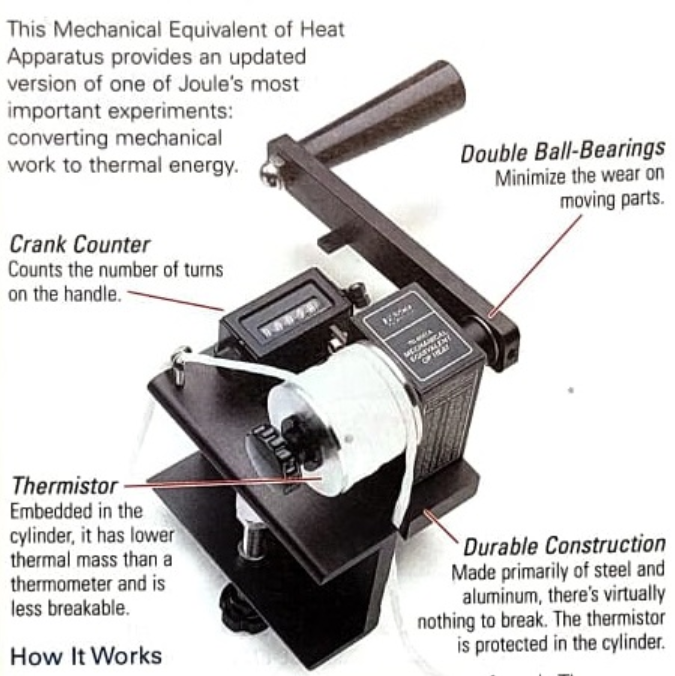
\includegraphics[scale=0.25]{pasco.png}
    \caption{Pasco TD8551A}
    \label{fig:pasco}
\end{figure}

\subsection{Equivalente eléctrico}
Por otro lado, los instrumentos utilizados para el montaje experimental fueron:

\begin{itemize}
    \item Calorímetro.
    \item Fuente de voltaje.
    \item Termopar. 
\end{itemize}

\begin{figure}[H]
    \centering
    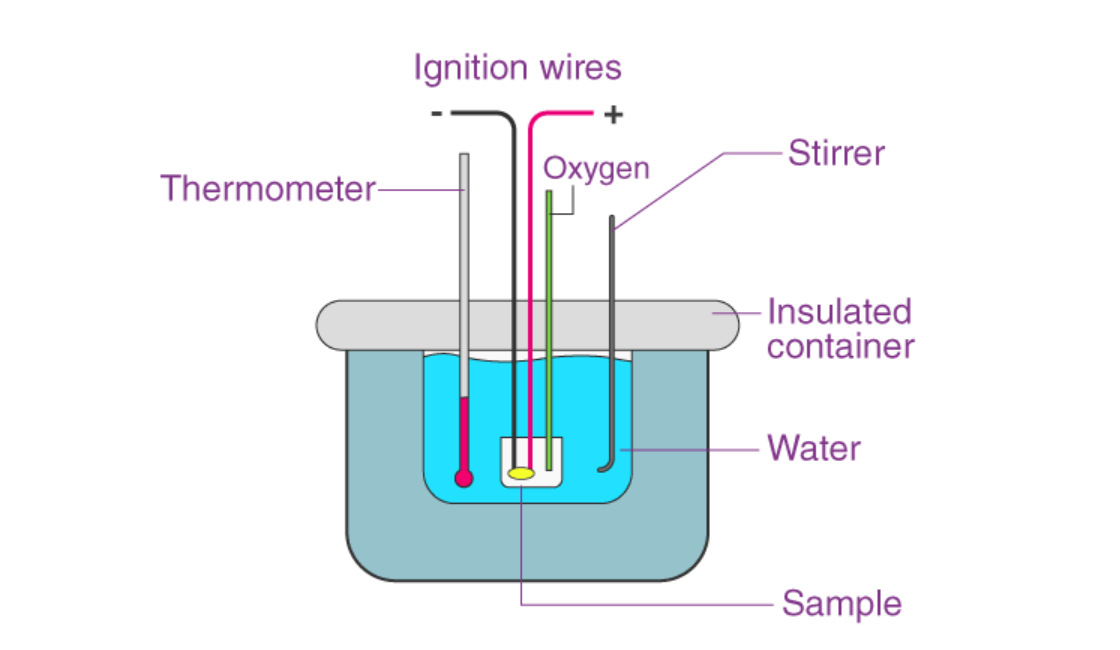
\includegraphics[scale=0.2]{calorimetro.png}
    \caption{Diagrama del calorímetro utilizado.}
    \label{fig:calorimetro}
\end{figure}

\subsubsection{Equivalente en agua del calorímetro}
La medición consiste en la mezcla de dos masas de agua aproximadamente iguales $M_0$ y $M_c$, una a temperatura ambiente $T_0$ y otra en su punto de ebullición $T_c$, y medir su temperatura de equilibrio $T_e$. Finalmente, se utiliza la expresión \ref{keq}.

\subsubsection{Equivalente eléctrico del calor}
Con un voltaje $V$ y corriente $I$ fijos, se introduce una cantidad $M$ de agua dentro del calorímetro; este tiene una resistencia que calentará el agua. Con la termocupla se anotan los cambios de temperatura en el tiempo.

\section{Resultados y análisis}

\subsection{Equivalente mecánico}
A continuación vemos las medidas experimentales correspondientes al equivalente mecánico.
\begin{figure}[H]
    \centering
    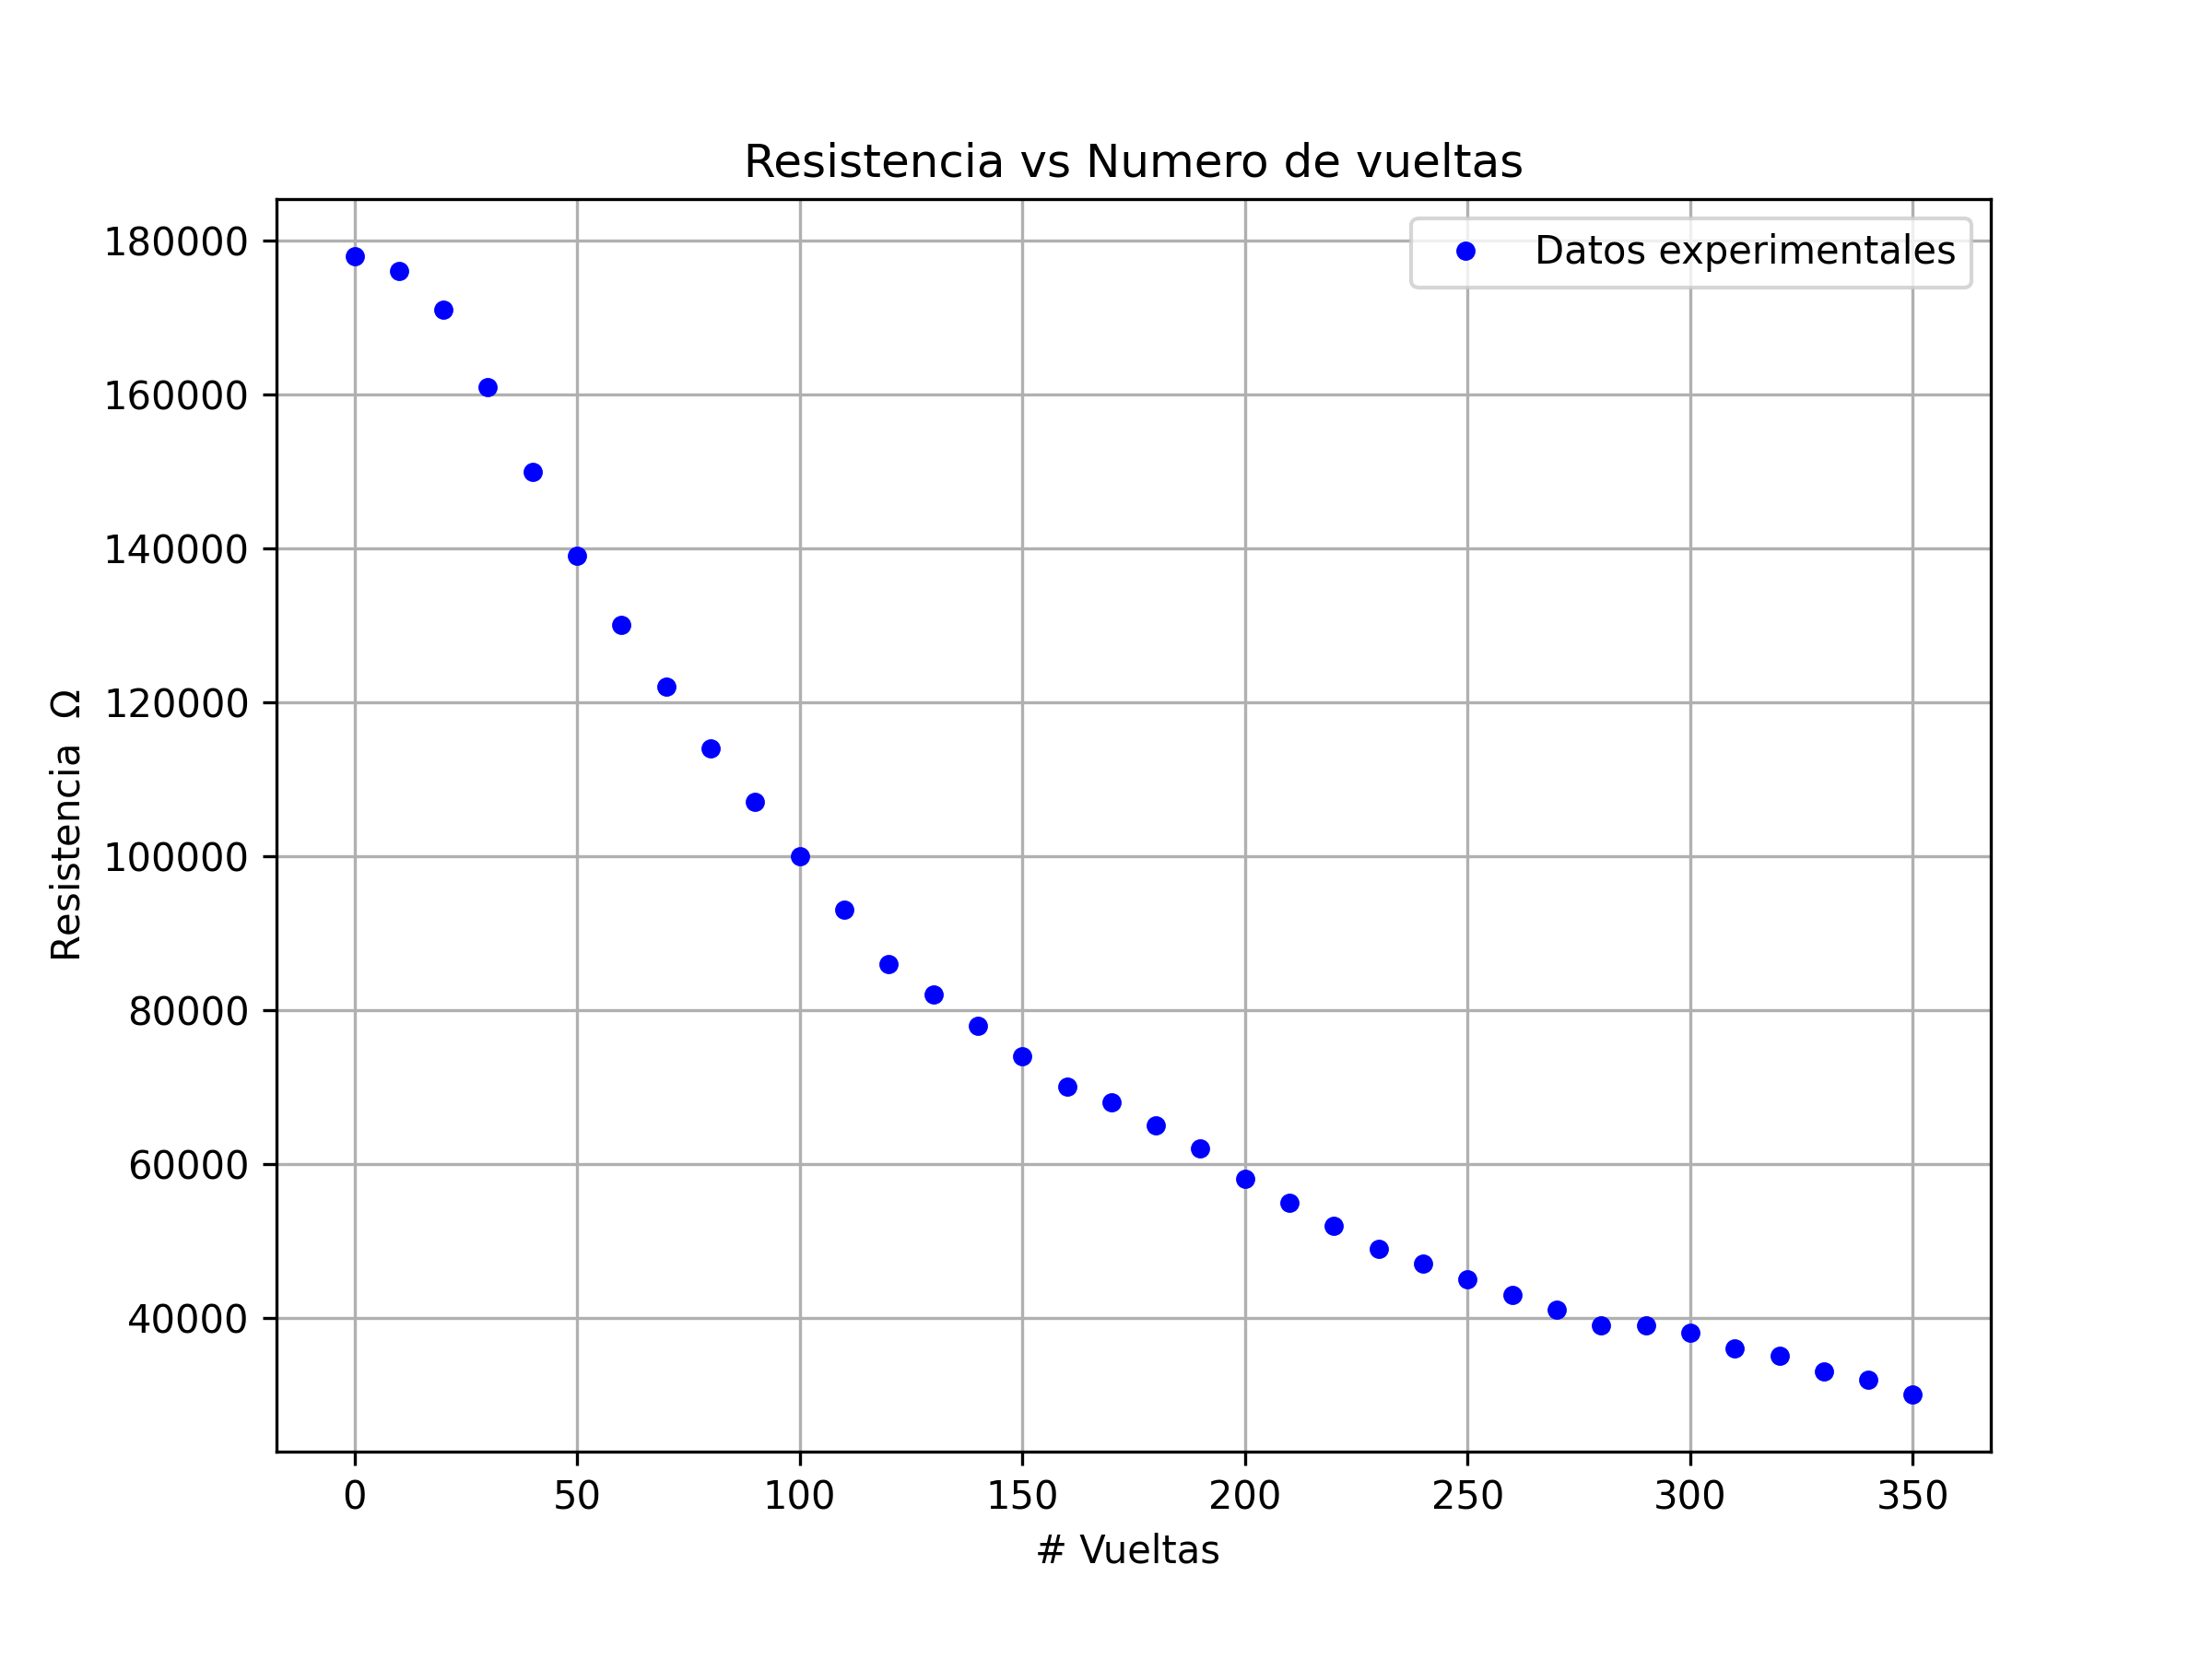
\includegraphics[scale=0.5]{RvsV.png}
    \caption{Relación entre resistencia y revoluciones del cilindro.}
    \label{fig:mecresrev}
\end{figure}
La medida está dada en resistencia pues, como se mencionó en la sección anterior, el termistor utilizado es del tipo NTC. Utilizando la tabla de conversión proporcionada por el fabricante\cite{pasco}, es posible realizar una regresión lineal al logaritmo de la resistencia. De este modo obtenemos una función continua de temperatura en función de resistencia y podemos encontrar el siguiente comportamiento de la resistencia en relación con el número de vueltas:
\begin{figure}[H]
    \centering
    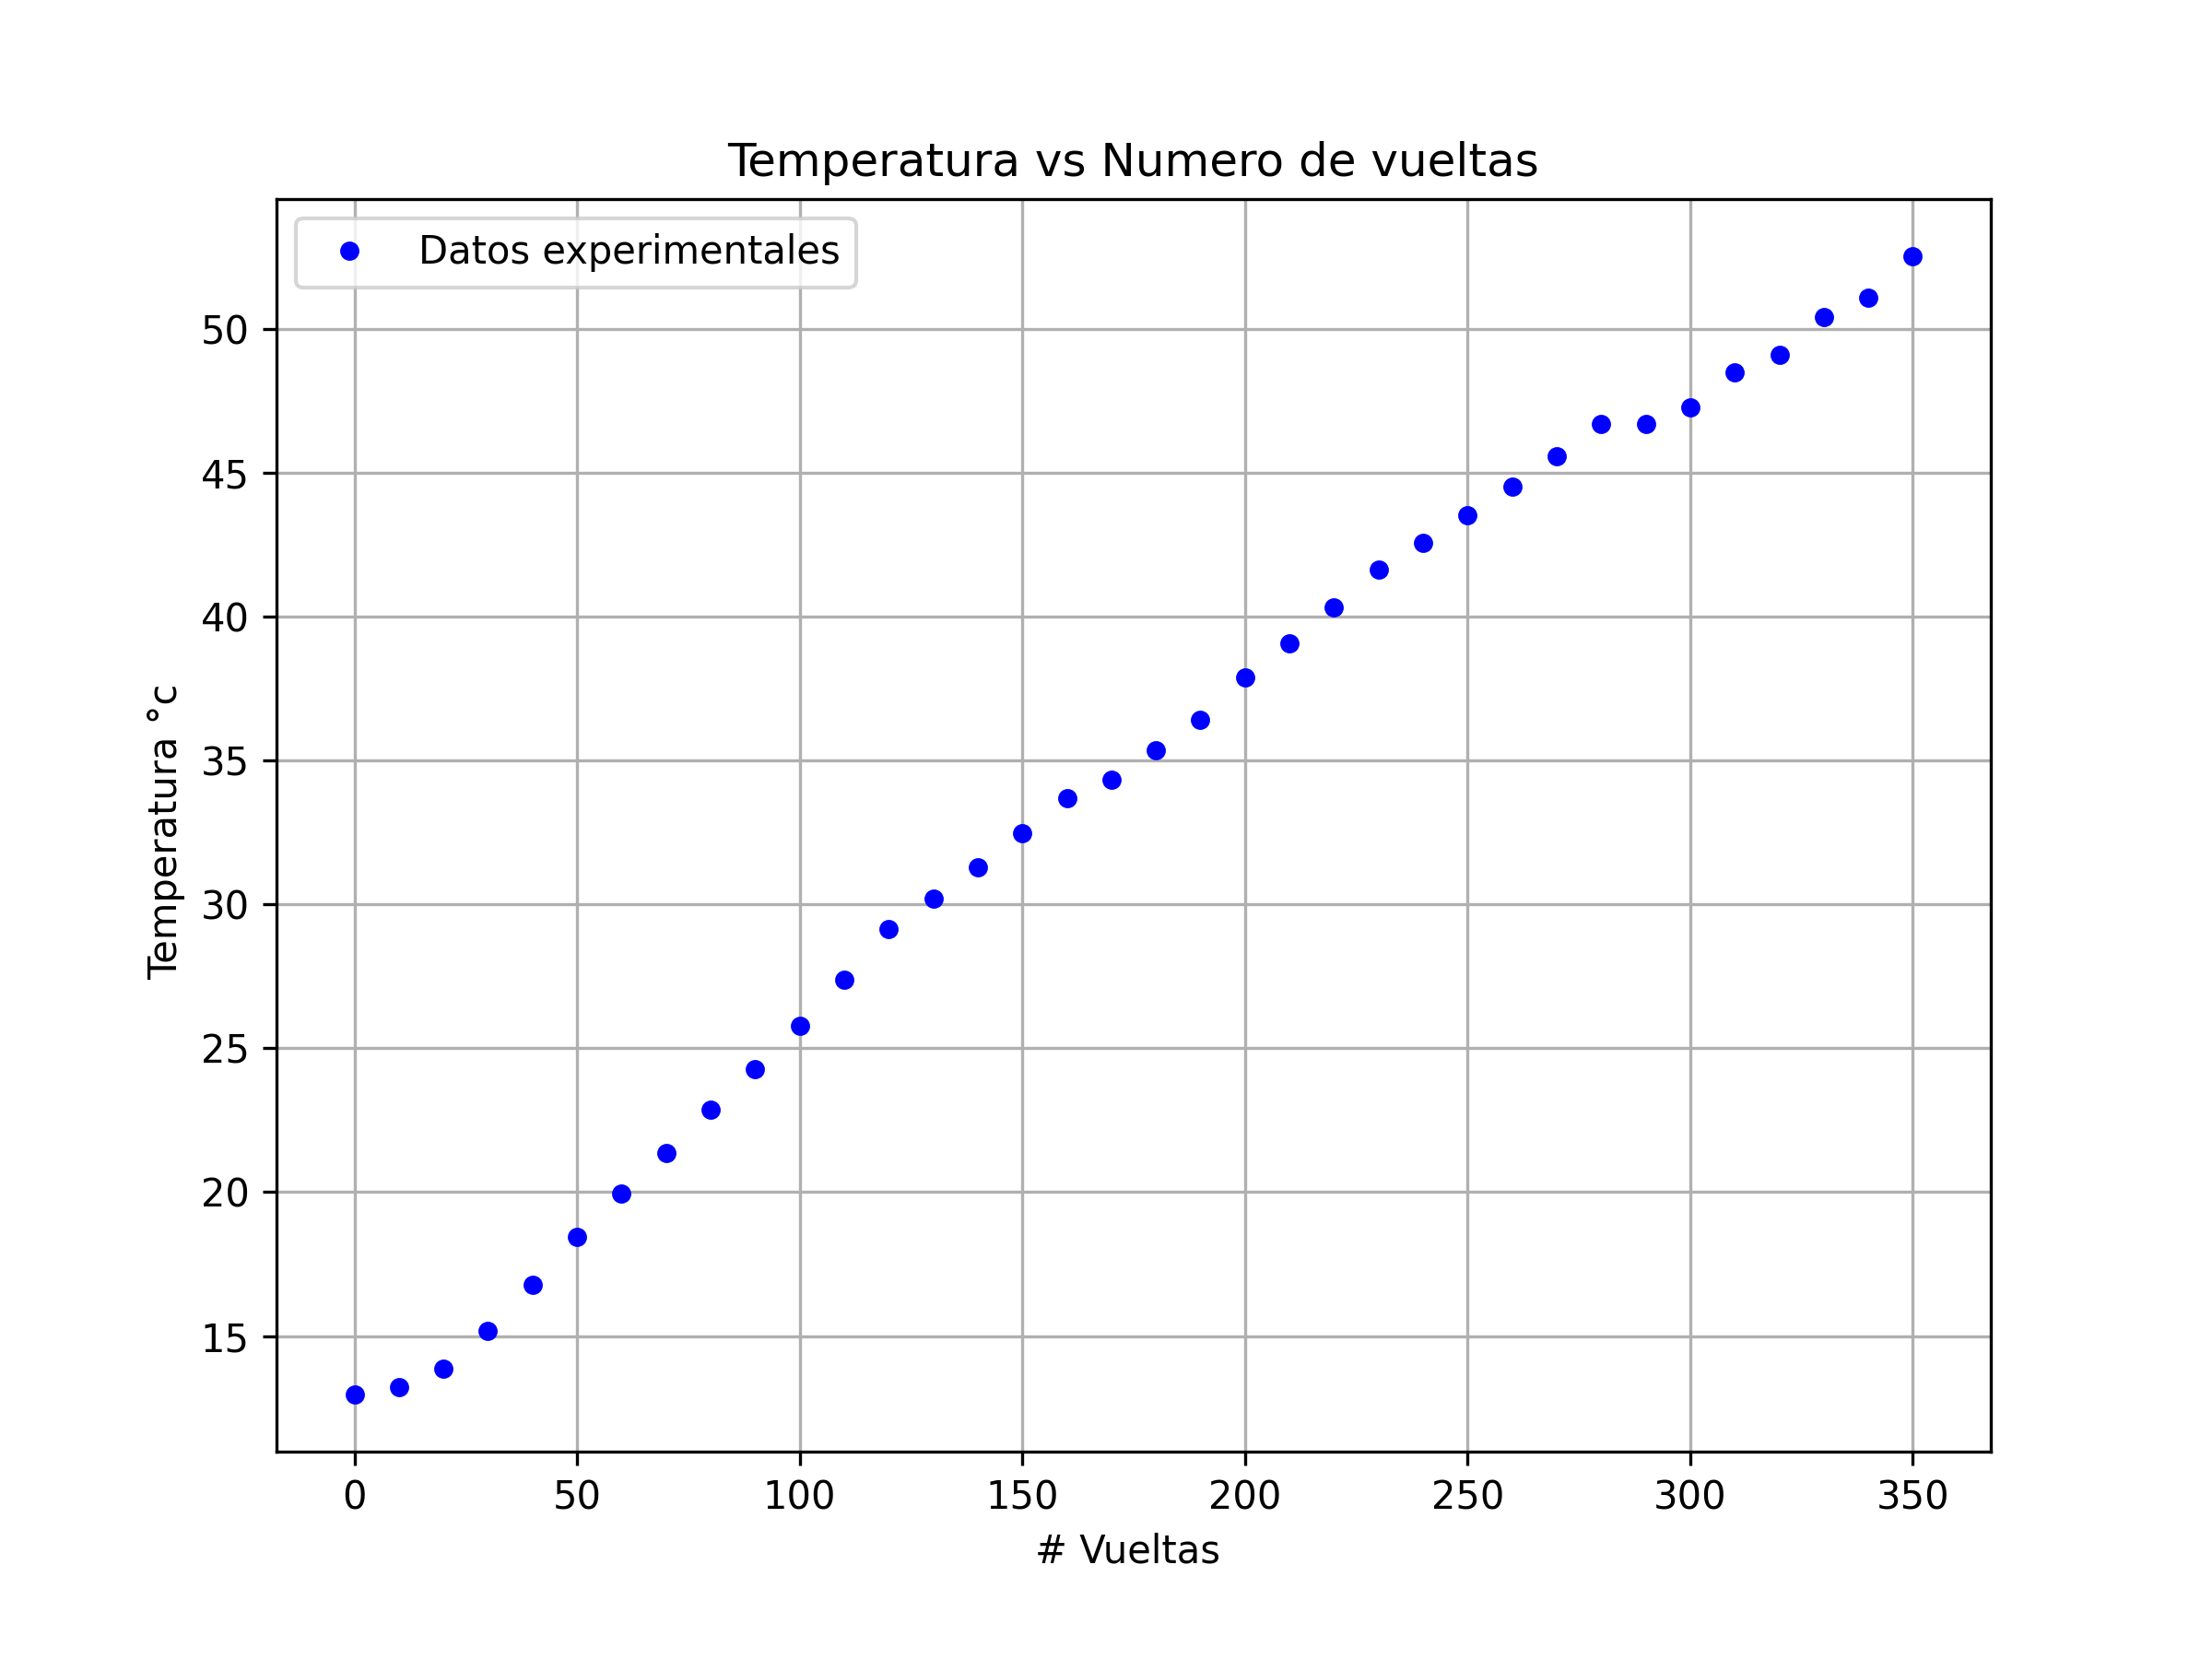
\includegraphics[scale=0.5]{TvsV.png}
    \caption{Relación entre temperatura y revoluciones del cilindro.}
    \label{fig:mectemprev}
\end{figure}
Habiendo convertido las temperaturas a Kelvin, utilizamos las ecuaciones \ref{eq:mecw} y \ref{eq:mecq} para calcular el trabajo mecánico sobre el sistema y el calor absorbido, respectivamente. Tenemos, entonces, el siguiente resultado:
\begin{figure}
    \centering
    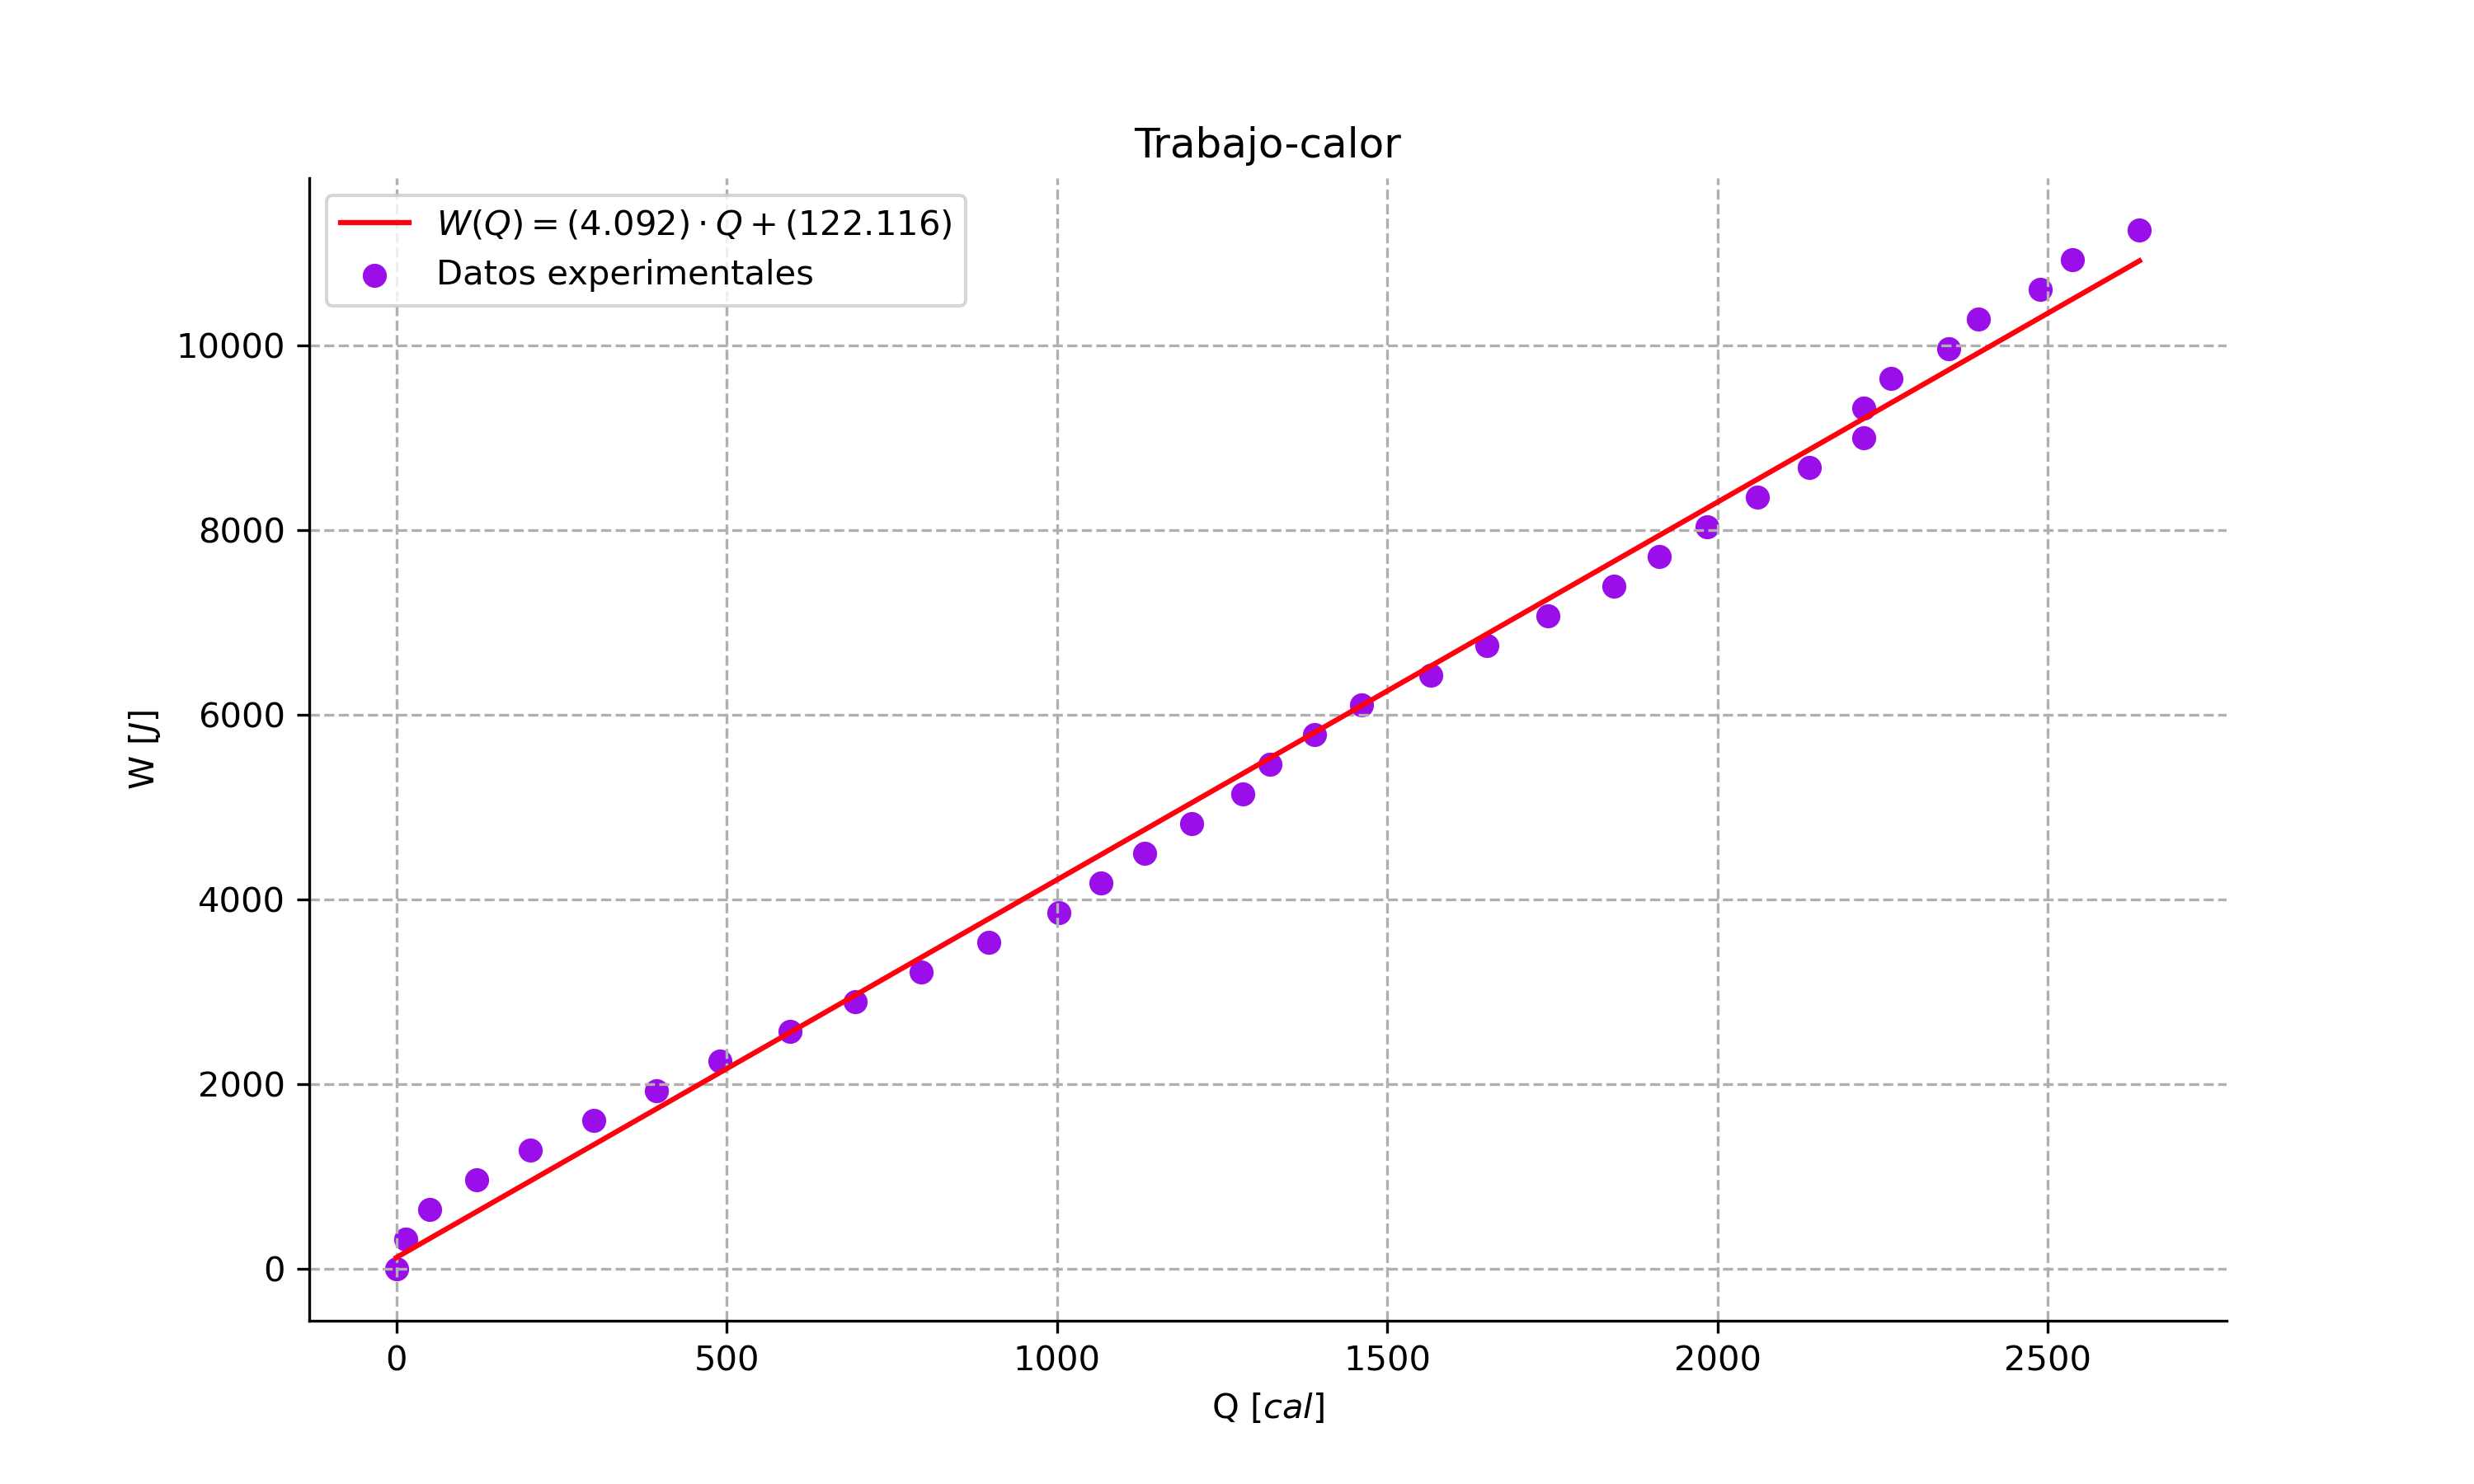
\includegraphics[scale=0.5]{mecworkheat.png}
    \caption{Relación entre el trabajo y el calor en el caso mecánico.}
    \label{fig:mecworkheat}
\end{figure}
Finalmente, conocemos que el equivalente mecánico del calor estará definido por:
\begin{equation}
    J = \frac{W}{Q}
    \label{eqivmec}
\end{equation}
Sabiendo esto, encontramos experimentalmente que el equivalente es:
\begin{equation*}
    J = 4.092 \frac{J}{cal}
\end{equation*}

\subsection{Equivalente eléctrico}
\subsubsection{Equivalente en agua del calorímetro}
En la siguiente tabla se resumen los datos recolectados:

\begin{table}[H]
\centering
\begin{tabular}{l|l}
$M_0$ & $(a \pm b)g$\\
$T_0$ & $(a \pm b) \degree C$a\\
$M_c$ & $(a \pm b)g$\\
$T_c$ & $(a \pm b) \degree C$\\
$T_e$ & $(a \pm b) \degree C$
\end{tabular}
\end{table}

Utilizando la expresión \ref{keq} y utilizando propagación de errores, tenemos:


\subsubsection{Equivalente eléctrico del calor}



\section{Conclusiones}
\subsection{Equivalente mecánico}
Se encontró experimentalmente el siguiente valor para el equivalente mecánico del calor:
\begin{equation*}
    J = 4.092 \frac{J}{cal}
\end{equation*}
Por otro lado, conocemos por la literatura\cite{pasco} que el valor esperado es $J = 4.184 \frac{J}{cal}$. De este modo, encontramos un error relativo porcentual de $\epsilon = 2.2\%$. Este error puede haber provenido de varios factores: por un lado, dado que el sistema no estaba completamente aislado, es posible que una parte del calor se haya cedido al ambiente; por otro lado, se encontraron dificultades a la hora de operar el TD8551A, con lecturas inconsistentes de resistencia e inestabilidad estructural al colgar las masas. 

\subsection{Equivalente eléctrico}



\begin{thebibliography}{X}

\bibitem{pasco} Instruction Manual and Experiment Guide for the PASCO scientific Model TD-8551A. \path{https://cdn.pasco.com/product_document/Mechanical-Equivalent-of-Heat-Apparatus-Manual-TD-8551A.pdf}

\bibitem{purcell} Edward M. Purcell, David J. Morin. Electricity and Magnetism (2013).

\bibitem{scehu} Curso Interactivo de Física en Internet. Calor específico de un sólido. \path{http://www.sc.ehu.es/sbweb/fisica3/calor/calorimetro/calorimetro.html}. 

 \end{thebibliography}

\end{document}